\section{Evaluation}
We evaluate the benefits of \oursys on a virtual environment in the Google Clod Platform(GCP).
For our testing we have crated three VMs; 16 core\footnote{These VMs have two threads per physical core} Intel Cascade Lake high-throughput VMs capable of 32Gb/s of  egress bandwidth\cite{gcp}, each with 64GB of RAM.

\subsection{Bifurcated TX}\label{sec:eval_bif}
In this experiment we evaluate the direct benefit of bifurcated system calls. Each program sends a UDP stream of 64 Byte packets. The goal of this experiment is to gauge the impact of system calls on perfromance. We compare a simple \texttt{send\_msg}, a kernel thread performing \texttt{kernel\_send\_msg} and \oursys. We run the naive version twice, once with \texttt{mitigations=off}\cite{mitigations} and once without this boot parameter. The results are shown in Fig \ref{fig:pps}. We see that \texttt{mitigations} have a negative impact of 20\% on the performance of the naive \texttt{send\_msg}. Without mitigations a kernel thread and \oursys beat the naive thread by 25\% and 20\% respectively.

\subsection{Zero Copy TX}
We evaluate the cost of data copying for single core and multi core sends. To minimise the impact of system calls on performance we send 256KB buffers. We evaluate a simple \texttt{send\_msg}, a \texttt{send\_msg} with \texttt{MSG\_ZERO\_COPY}, \textcolor{red}{\texttt{sendfile}} and \oursys.

\begin{figure}[t]
    \centering
    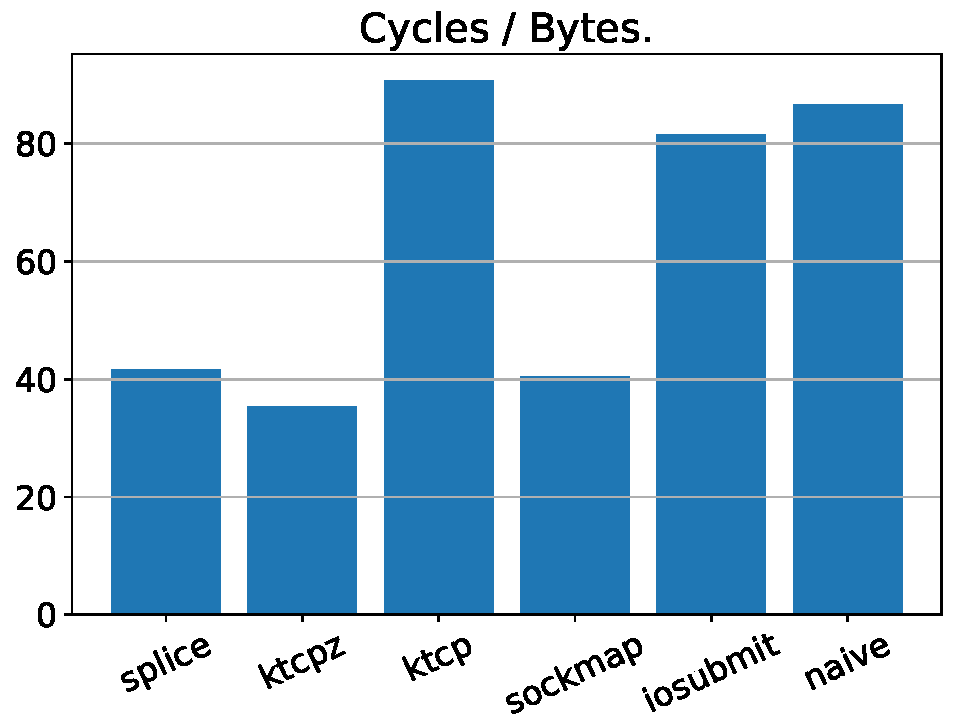
\includegraphics[width=\columnwidth]{Figure_1.pdf}
    \caption{The average cycles per packet need for each splicing solution; taken over 10 iterations runs }
    \label{fig:cyc_byte}
\end{figure}
\begin{figure}[t]
    \centering
    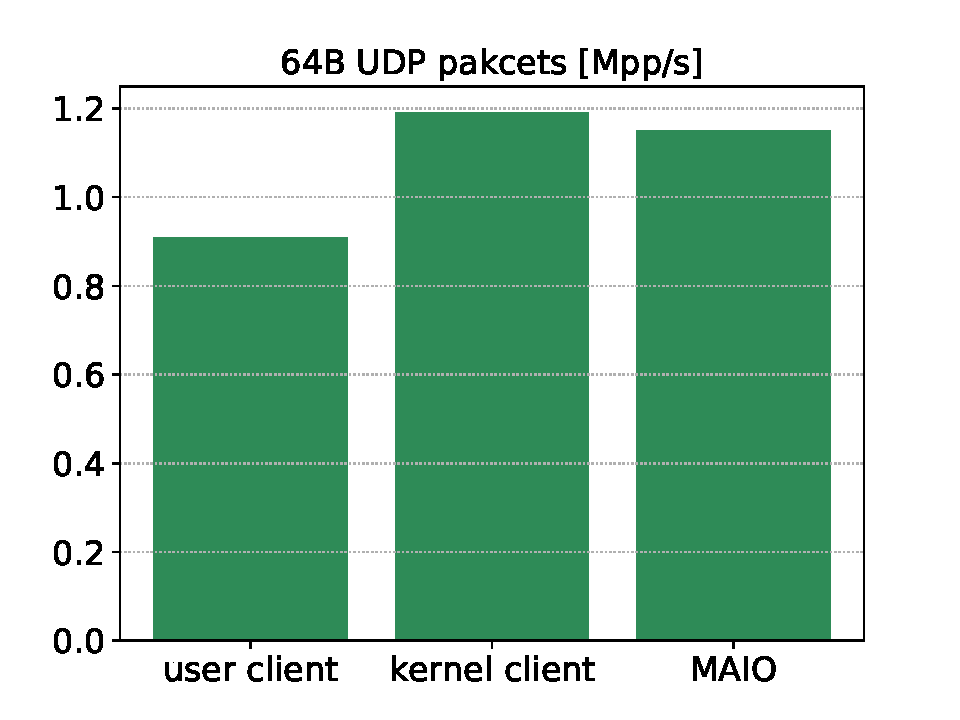
\includegraphics[width=\columnwidth]{bifurcated.pdf}
    \caption{Number of 64B udp packets sent using user-space sockets(both with and without mitigations), kernel sockets and MAIO.} 
    \label{fig:pps}
\end{figure}
\begin{figure}[t]
    \centering
    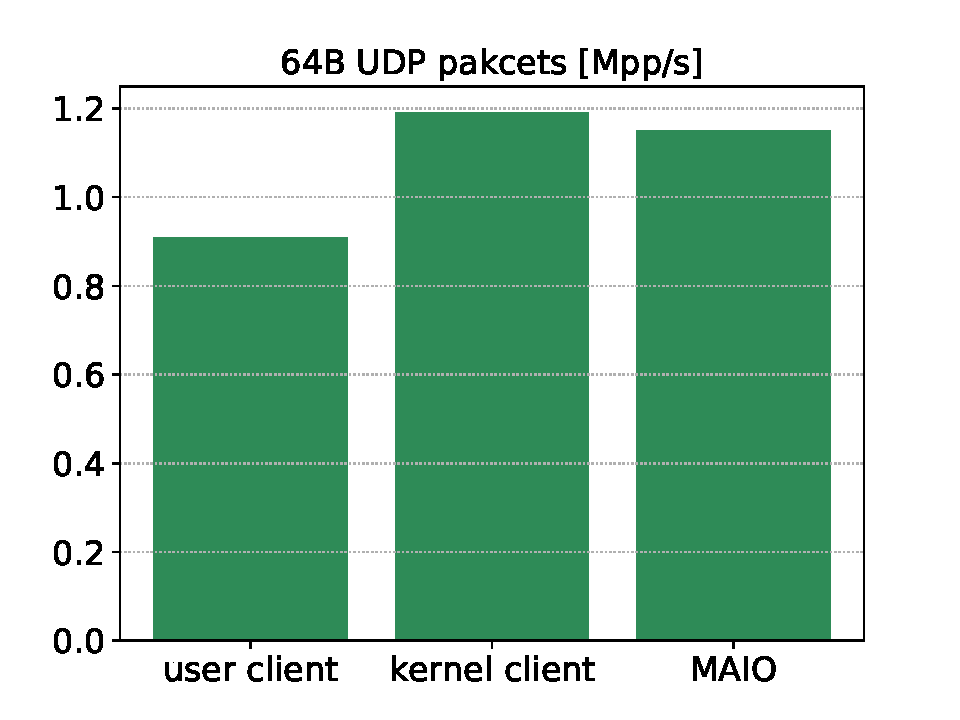
\includegraphics[width=\columnwidth]{bifurcated.pdf}
    \caption{\textcolor{red}{Placeholder}}
    \label{fig:tx_compare}
\end{figure}
\subsection{Socket Splicing}
We perform a simple TCP socket splicing experiment (i.e., Mvoing bytes from one TCP socket to another) akin to the TCP-split functionality of KTCP. We measure the effectiveness of each proposed solution by looking the the number of CPU cycles spent on average to splice (i.e., receive and send) a single byte.

We use 256KB buffers both for RX and TX, rendering the effect of system calls negligible. System calls account for less than 1\% of the cpu syscalls of iosubmit,splice and naive. We use perf\cite{perf} to analyze the major contributors to the cycles per byte costs of each of tested techniques. Unsurprisingly, KTCP, iosubmit and naive all spend between 25\% to 32\% of the cycles on memory copying. Results are shown in Fig. \ref{fig:cyc_byte}. While both splice and sockmap perform much better than the copying functions \oursys is still able outperform both by about 10\%.

%Why we are \emph{not} touching DPDK and friends with a stick.

%Splice Compare (Check Poll):
%\begin{itemize}
%    \item Naive
%    \item SOCKMAP
%    \item splice
%    \item vmsplice  (?)
%    \item io\_remap (?)
%    \item ktcp - kernel TCP client + halfduplex.
%    \item \oursys - kernel zero TCP client + read/write op. 
%    \item ktcp\_zero. - kernel zero TCP client
%\end{itemize}


%\subsection{BW - cycles/byte}
%\subsection{Latency TCP/RR}
%\subsection{Scale - multiple connections - BW,Latency}